\documentclass[14pt, a4paper]{article}
\usepackage{minitoc}
\usepackage[left=3.00cm, right=2.5cm, top=2.00cm, bottom=2.00cm]{geometry}
\usepackage{amsmath}
\usepackage{amssymb}
\usepackage{amsthm}
\usepackage{mathtools}
\usepackage{graphicx}
%\usepackage{algpseudocode}
%\usepackage{algorithm}
\usepackage[ruled,vlined,linesnumbered]{algorithm2e}
\usepackage{blindtext}
\usepackage{setspace}
\usepackage[utf8]{inputenc}
\usepackage[utf8]{vietnam}
\usepackage[center]{caption}
\usepackage[shortlabels]{enumitem}
\usepackage{fancyhdr} % header, footer
\usepackage{hyperref} % loại bỏ border với mục lục và công thức
\usepackage[nonumberlist, nopostdot, nogroupskip]{glossaries}
\usepackage{glossary-superragged}
\usepackage{tikz,tkz-tab}
\usepackage{pythonhighlight}
\setglossarystyle{superraggedheaderborder}
\pagestyle{fancy}
%\usepackage[style=numeric,sortcites]{biblatex}
%\addbibresource{ref.bib}
%\usepackage[numbers]{natbib}
\usepackage{indentfirst}
\usepackage[natbib,backend=biber,style=ieee, sorting=ynt]{biblatex}

\usepackage{caption}
\usepackage{subcaption}

\bibliography{ref.bib}

\graphicspath{{./figures/}}

\fancyhf{}
%\rhead{\textbf{Môn học: Các phương pháp thống kê hiện đại trong nghiên cứu Xã hội học}}
\lhead{\textbf{GVHD: TS. Trịnh Quốc Anh}}
\rfoot{\thepage}
\lfoot{\textbf{Học viên thực hiện: Nguyễn Chí Thanh - 21007925}}
\renewcommand{\headrulewidth}{0.4pt}
\renewcommand{\footrulewidth}{0.4pt}
%
%\numberwithin{equation}{section}
%\numberwithin{algorithm}{section}
%\numberwithin{figure}{section}
%
%\setlength{\parindent}{0.5cm}
%
%\setcounter{secnumdepth}{3} % Cho phép subsubsection trong report
%\setcounter{tocdepth}{3} % Chèn subsubsection vào bảng mục lục

%\newtheorem{dl}{Định lý}
%\newtheorem{md}{Mệnh đề}
%\newtheorem{bd}{Bổ đề}
%\newtheorem{dn}{Định nghĩa}
%\newtheorem{hq}{Hệ quả}

%\newtheorem{baitap}{Bài tập}
%\newtheorem*{loigiai}{Lời giải}

%\numberwithin{dl}{section}
%\numberwithin{md}{section}
%\numberwithin{bd}{section}
%\numberwithin{dn}{section}
%\numberwithin{hq}{section}

\setlength{\parindent}{0cm}

\newtheorem{dl}{Định lý}
\newtheoremstyle{sltheorem}
{}                % Space above
{}                % Space below
{\normalfont}        % Theorem body font % (default is "\upshape")
{}                % Indent amount
{\bfseries}       % Theorem head font % (default is \mdseries)
{.}               % Punctuation after theorem head % default: no punctuation
{ }               % Space after theorem head
{}                % Theorem head spec
\theoremstyle{sltheorem}
\newtheorem{baitap}{Bài tập}
\newtheoremstyle{soltheorem}
{}                % Space above
{}                % Space below
{\normalfont}        % Theorem body font % (default is "\upshape")
{}                % Indent amount
{\bfseries}       % Theorem head font % (default is \mdseries)
{.}               % Punctuation after theorem head % default: no punctuation
{\newline}               % Space after theorem head
{}                % Theorem head spec
\theoremstyle{soltheorem}
\newtheorem*{loigiai}{Lời giải}

\onehalfspacing


\begin{document}
\begin{titlepage}

    \newcommand{\HRule}{\rule{\linewidth}{0.5mm}} % Defines a new command for the horizontal lines, change thickness here

    \center % Center everything on the page

    %----------------------------------------------------------------------------------------
    %	HEADING SECTIONS
    %----------------------------------------------------------------------------------------
    \textsc{\LARGE Đại học Quốc Gia Hà Nội}\\[0.5cm]
    \textsc{\LARGE Trường đại học Khoa học tự nhiên}\\[0.5cm] % Name of your university/college
    \textsc{\LARGE Khoa Toán - Cơ - Tin học}\\[0.5cm]

    
\includegraphics[scale=0.2]{HUS-logo.jpg}\\[0.5cm]

    \textsc{\Large Chuyên ngành: Khoa học dữ liệu}\\[0.5cm] % Major heading such as course name


    %----------------------------------------------------------------------------------------
    %	TITLE SECTION
    %----------------------------------------------------------------------------------------

    \HRule \\[0.4cm]
    { \huge \bfseries Bài tập môn học}\\[0.4cm] % Title of your document
    \HRule \\[1.5cm]

    \textsc{\Large Môn học: Các phương pháp thống kê hiện đại \\ trong nghiên cứu Xã hội học}\\[1cm] % Minor heading such as course title


    \textsc{\Large Bài tập số 2}\\[1cm]


    %----------------------------------------------------------------------------------------
    %	AUTHOR SECTION
    %----------------------------------------------------------------------------------------
    \begin{minipage}{0.4\textwidth}
        \begin{flushleft} \large
        \emph{Giảng viên hướng dẫn:} \\
        TS. Trịnh Quốc Anh % Supervisor's Name
        \end{flushleft}
    \end{minipage}\\[0.5cm]

    \begin{minipage}{0.4\textwidth}
    \begin{flushleft} \large
    \emph{Học viên thực hiện:}\\
    Nguyễn Chí Thanh \\
    MSHV: 21007925 \\ % Your name
    Lớp: Khoa học dữ liệu - K4
    \end{flushleft}
    \end{minipage}


    % If you don't want a supervisor, uncomment the two lines below and remove the section above
    %\Large \emph{Author:}\\
    %John \textsc{Smith}\\[3cm] % Your name

    %----------------------------------------------------------------------------------------
    %	DATE SECTION
    %----------------------------------------------------------------------------------------

    % I don't want day because it is English
    % {\large \today}\\[2cm] % Date, change the \today to a set date if you want to be precise

    %----------------------------------------------------------------------------------------
    %	LOGO SECTION
    %----------------------------------------------------------------------------------------

    %\includegraphics{logo/rsz_3logo-khtn.png}\\[1cm] % Include a department/university logo - this will require the graphicx package

    %----------------------------------------------------------------------------------------

    \vfill % Fill the rest of the page with whitespace

\end{titlepage}

\nocite{*}

\newpage

\begin{baitap}
    Dữ liệu Sonar là dữ liệu gì và hãy mô tả thống kê các thông tin thu thập được.
\end{baitap}

\begin{loigiai}
    Dữ liệu Sonar là dữ liệu gì và hãy mô tả thống kê các thông tin thu thập được.
    \begin{itemize}
        \item Dữ liệu Sonar là dữ liệu gì
        Tập dữ liệu Sonar là tập dữ liệu được Gorman và Sejnowski sử dụng trong công trình nghiên cứu phân loại tín hiệu sonar sử dụng mạng neuron \cite{gorman1988analysis}.
        Nhiệm vụ của bài toán là huấn luyện một mạng neuron để phân biệt tín hiệu sonar thu được từ một hình trụ kim loại hay một hình trụ đá thô.
        
        Mỗi phần tử trong tập dữ liệu gồm tập 60 số trong khoảng từ 0.0 đến 1.0.
        Từng số biểu diễn năng lượng trong một dải tần số nhất định được tính trong một khoảng thời gian nhất định. 
        Từng nhãn liên kết với từng phần tử bao gồm chữ cái "R" nếu tín hiệu thu được hình trụ đá thô và "M" nếu tín hiệu thu được từ hình trụ kim loại.
        Các số trong nhãn theo thứ tự tăng dần góc thu được tín hiệu nhưng thông tin về góc không được đưa trực tiếp vào trong tập dữ liệu.
        \item Mô tả thống kê các thông tin thu tập được:
        
        Ta kiểm tra tính chuẩn của dữ liệu, ta giả thiết $H_0$ là dữ liệu theo phân phối chuẩn và đối thiết $H_1$ dữ liệu không theo phân phối chuẩn.

        Ta chọn các số $\alpha$:

        \begin{equation*}
            0 < \alpha_1 < \alpha_2 < \dots < \alpha_m < 1, m = 20
        \end{equation*}

        Các số $\alpha_i, i = 1,\dots,m$ là số cách đều nhau và $\alpha_1=0.01, \alpha_{20}=0.99$

        Ta tìm các số $c^2$:

        \begin{equation*}
            \infty > c_1^2 > c_2^2 > \dots > c_m^2 > 0
        \end{equation*}

        với $c_i^2 = \chi_{60}^2 (\alpha_i)$

        Theo lý thuyết ta có:
        \begin{equation*}
            \begin{aligned}
                &p(\bold{x}_i \in V(c^2)) = 1 - \alpha_c \\
                &V(c^2) = \lbrace \bold{x} \vert (\bold{x} - \bold{\mu})^T \bold{\Sigma}^{-1} (\bold{x} - \bold{\mu}) \leq c^2 \rbrace
            \end{aligned}
        \end{equation*}

        \begin{equation*}
            \begin{aligned}
                p(\bold{x} \in \Omega \backslash V(c_1^2)) &= \alpha_1 \\
                p(\bold{x} \in V(c_1^2) \backslash V(c_2^2)) &= \alpha_2 - \alpha_1 \\
                &\dots \\
                p(\bold{x} \in V(c_{m-1}^2) \backslash V(c_m^2)) &= \alpha_m - \alpha_{m-1} \\
                p(\bold{x} \in V(c_m^2)) &= 1 - \alpha_m
            \end{aligned}
        \end{equation*}

        Từ dữ liệu thực tế:
        \begin{equation*}
            \begin{aligned}
                n_1 &= \lvert \lbrace \bold{x}_i \vert \bold{x}_i \in \Omega \backslash V(c_1^2) \rbrace \rvert \\
                n_2 &= \lvert \lbrace \bold{x}_i \vert \bold{x}_i \in V(c_1^2) \backslash V(c_2^2) \rbrace \rvert \\
                &\dots \\
                n_{m+1} &= \lvert \lbrace \bold{x}_i \vert \bold{x}_i \in  V(c_m^2) \rbrace \rvert \\
            \end{aligned}
        \end{equation*}

        với:

        \begin{equation*}
            \begin{aligned}
                n_1 &= \lvert \lbrace \bold{x}_1 \vert \bold{x}_1 \in \Omega \backslash V(c_1^2) \rbrace \rvert \\
                &=\lvert \lbrace \bold{x}_1 \vert (\bold{x}_1 - \bold{\mu})^T \bold{S}^{-1} (\bold{x}_1 - \bold{\mu}) > c^2  \rbrace \rvert
            \end{aligned}
        \end{equation*}
    \end{itemize}

    Ta tính các quan sát:

    \begin{equation*}
        O_i = \dfrac{n_i}{n}, i=1, \dots, m+1
    \end{equation*}

    Ta tính test thống kê:

    \begin{equation*}
        T = \sum_{i=1}^{m+1} \dfrac{(O_i - E_i)^2}{E_i}
    \end{equation*}

    Ta bác bỏ $H_0$ nếu $T > \chi_m^2(\alpha)$

    Ta sử dụng code:

    \begin{python}
import pandas as pd
import numpy as np
from scipy.stats import chi2
import seaborn as sns

y = df["Class"]
x = df.drop("Class", axis=1).to_numpy()
mean_x = np.mean(x, axis=0)
S = np.matmul((x - mean_x[np.newaxis, :]).T, x - mean_x[np.newaxis, :]) / (x.shape[0] - 1)
inverted_S = np.linalg.inv(S)
alphas = np.linspace(0.01, 0.99, num=20)
c_sqr = chi2.ppf(1-alphas, x.shape[1])
alphas = np.insert(alphas, 0, 0)
alphas = np.append(alphas, 1)
alpha_diff = np.diff(alphas)
stat_test = ((x - mean_x[np.newaxis, :]).dot(inverted_S) * (x - mean_x[np.newaxis, :])).sum(axis=1)
observed = np.zeros(alpha_diff.shape[0], dtype=np.uint8)
for el in stat_test:
    for i in range(alpha_diff.shape[0]):
        if i == 0:
            if el >= c_sqr[i]:
                observed[i] += 1
                #print(i, el, c_sqr[i])
                break
        elif i > 0 and i < (alpha_diff.shape[0] - 1):
            if el >= c_sqr[i] and el < c_sqr[i-1]:
                observed[i] += 1
                #print(i, el, c_sqr[i-1], c_sqr[i])
                break
        else:
            if el < c_sqr[i-1]:
                observed[i] += 1
                break
            
                
observed = observed/np.sum(observed)
observed, np.sum(observed)
chi_test = np.sum((alpha_diff - observed)**2/alpha_diff)
chi_test, chi2.ppf(0.95, alphas.shape[0])
    \end{python}
    
    Ta tính được $T=11.03288$ và $\chi_20^2(0.05)=33.9244$, vậy $T < \chi_20^2(0.05)$, ta chưa có cơ sở bác bỏ $H_0$ vậy dữ liệu là phân phối chuẩn nhiều chiều.

    \begin{figure}[h!]
        \centering
        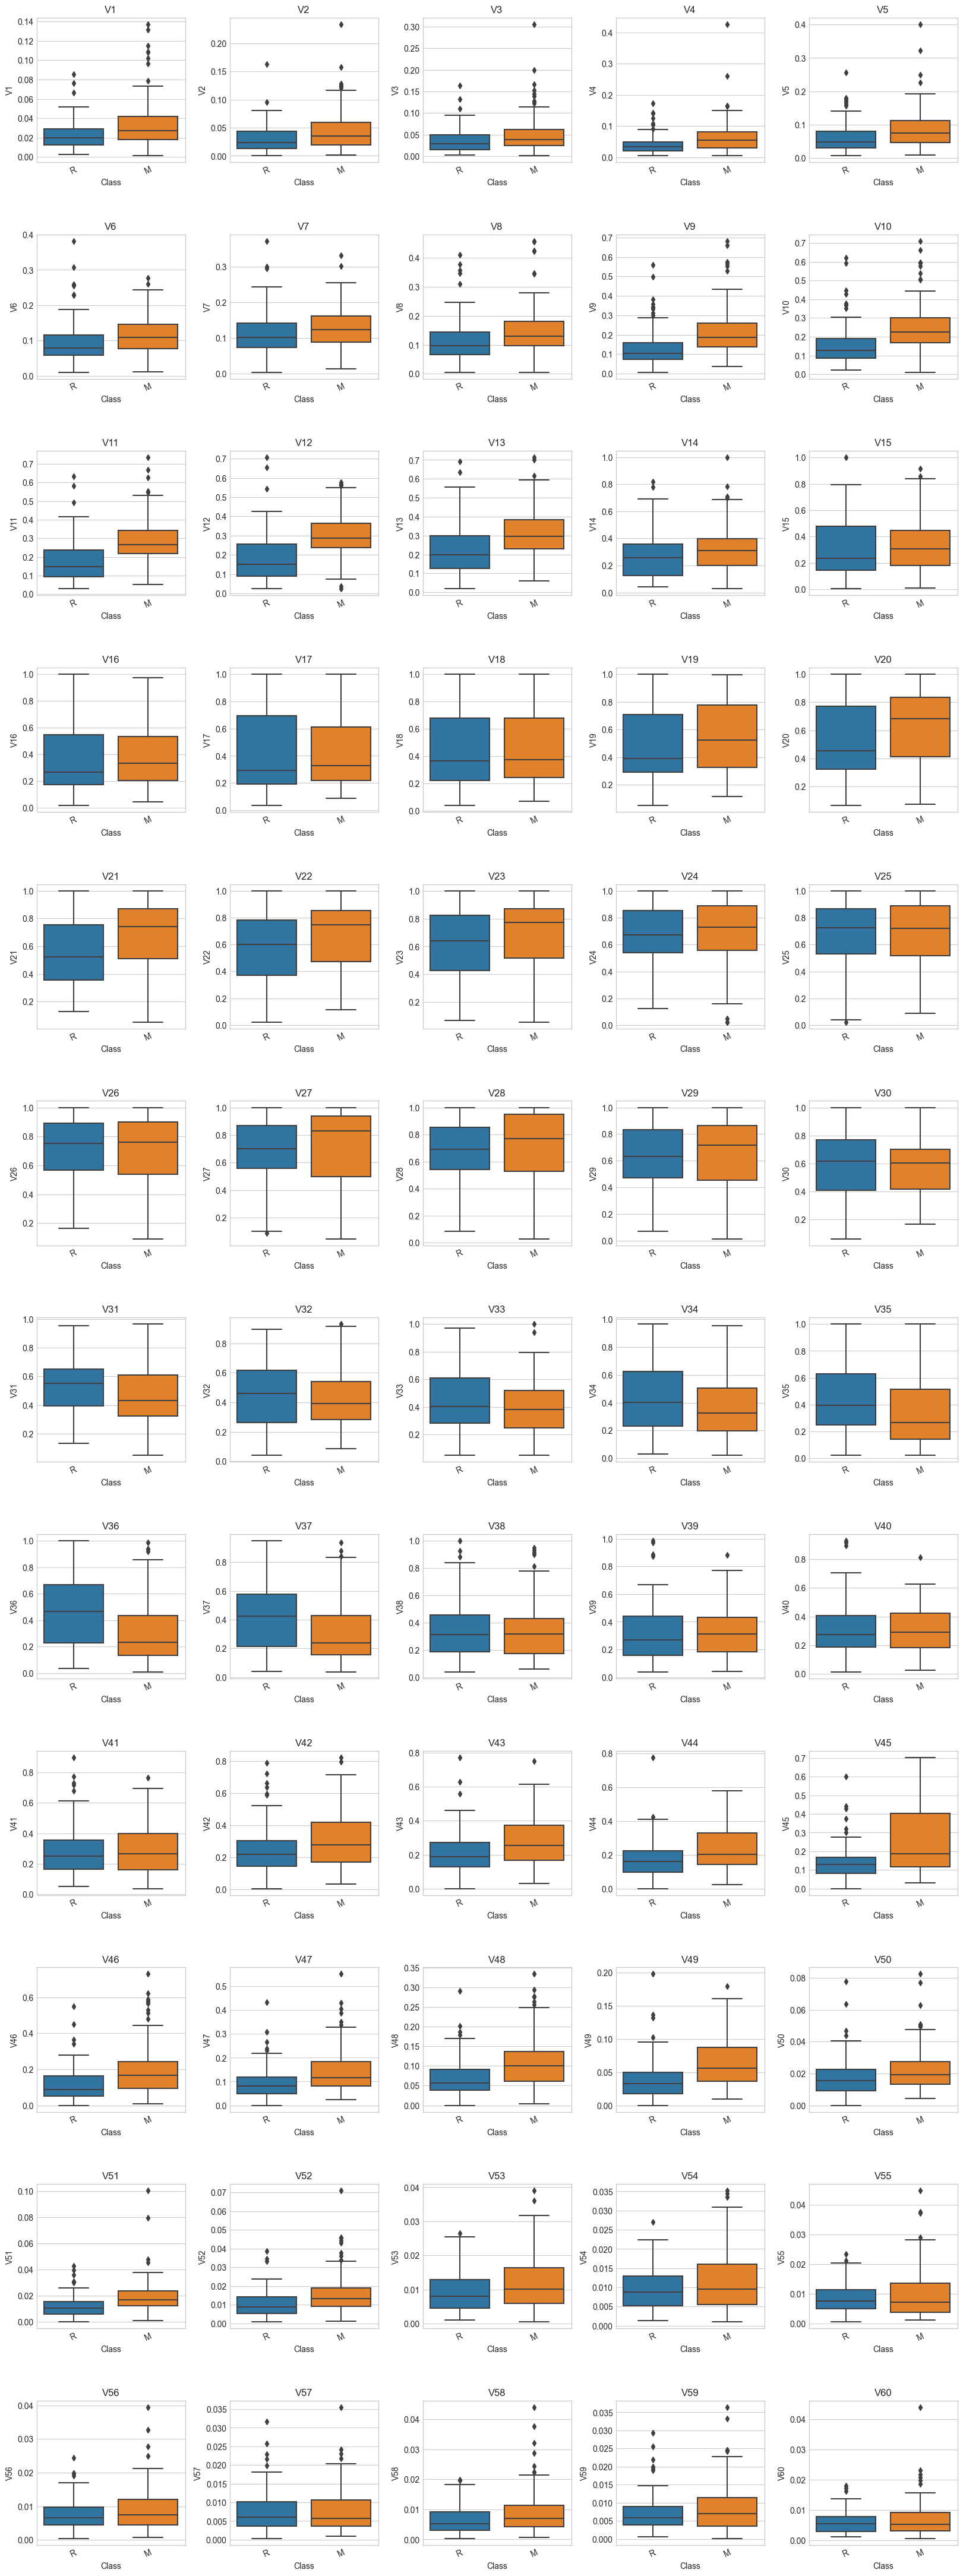
\includegraphics[scale=0.2]{box_plot.png}
        \caption{Boxplot của các biến theo từng loại vật liệu của hình trụ}
        \label{fig:box_plot}
    \end{figure}

    Hình \ref{fig:box_plot} biểu diễn boxplot của từng biến theo từng loại vật liệu của hình trụ.
    Ta nhận thấy trong từng biến, phân phối của hai nhãn không có quá nhiều sự khác biệt.

    \begin{figure}[h!]
        \centering
        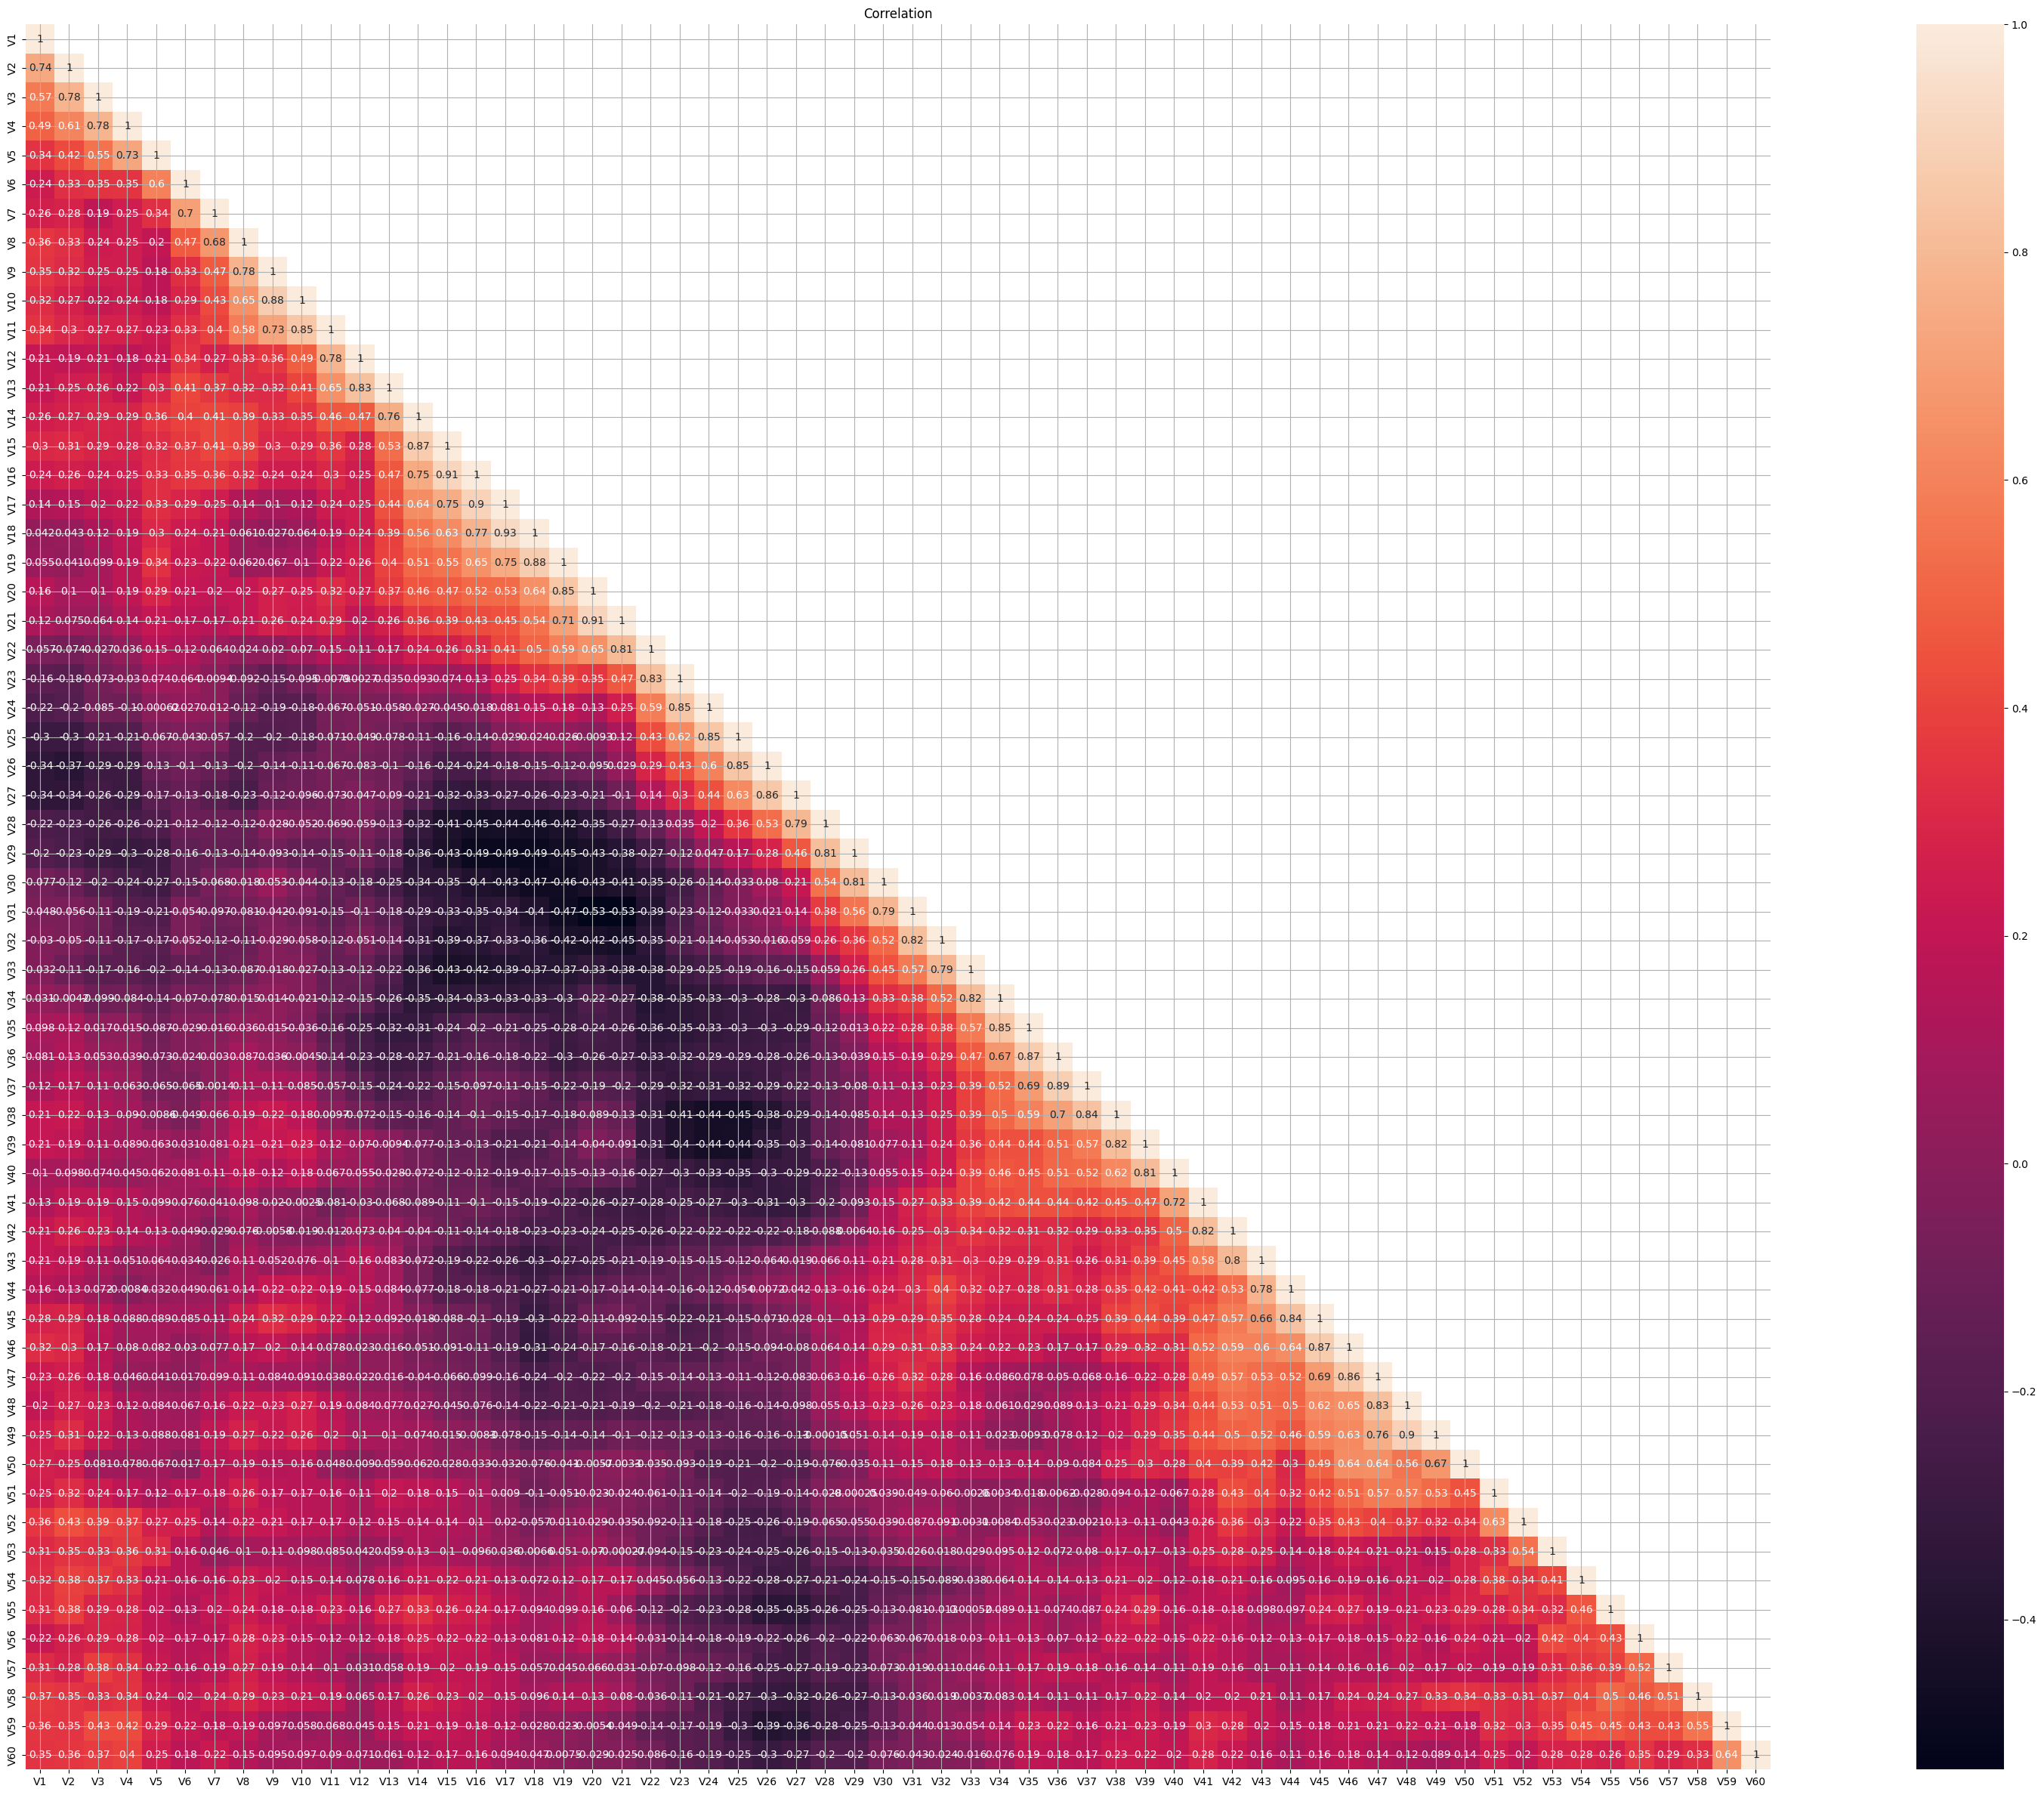
\includegraphics[scale=0.2]{correl_heatmap.png}
        \caption{Độ tương quan của đôi một các biến}
        \label{fig:correl_heatmap}
    \end{figure}

    Hình \ref{fig:correl_heatmap} biểu diễn độ tương quan của đôi một từng cặp biến.
    Các biến ở cạnh nhau có độ tương quan khá lớn, lý do các dải tần số gần nhau cũng sẽ có năng lượng tương đối giống nhau.
    Những dải tần số cách nhau khoảng 10 dải thường có độ tương quan âm.
    Những dài tần số cách nhau hơn 10 dải thường có độ tương quan tương đối thấp.

    \begin{figure}[h!]
        \centering
        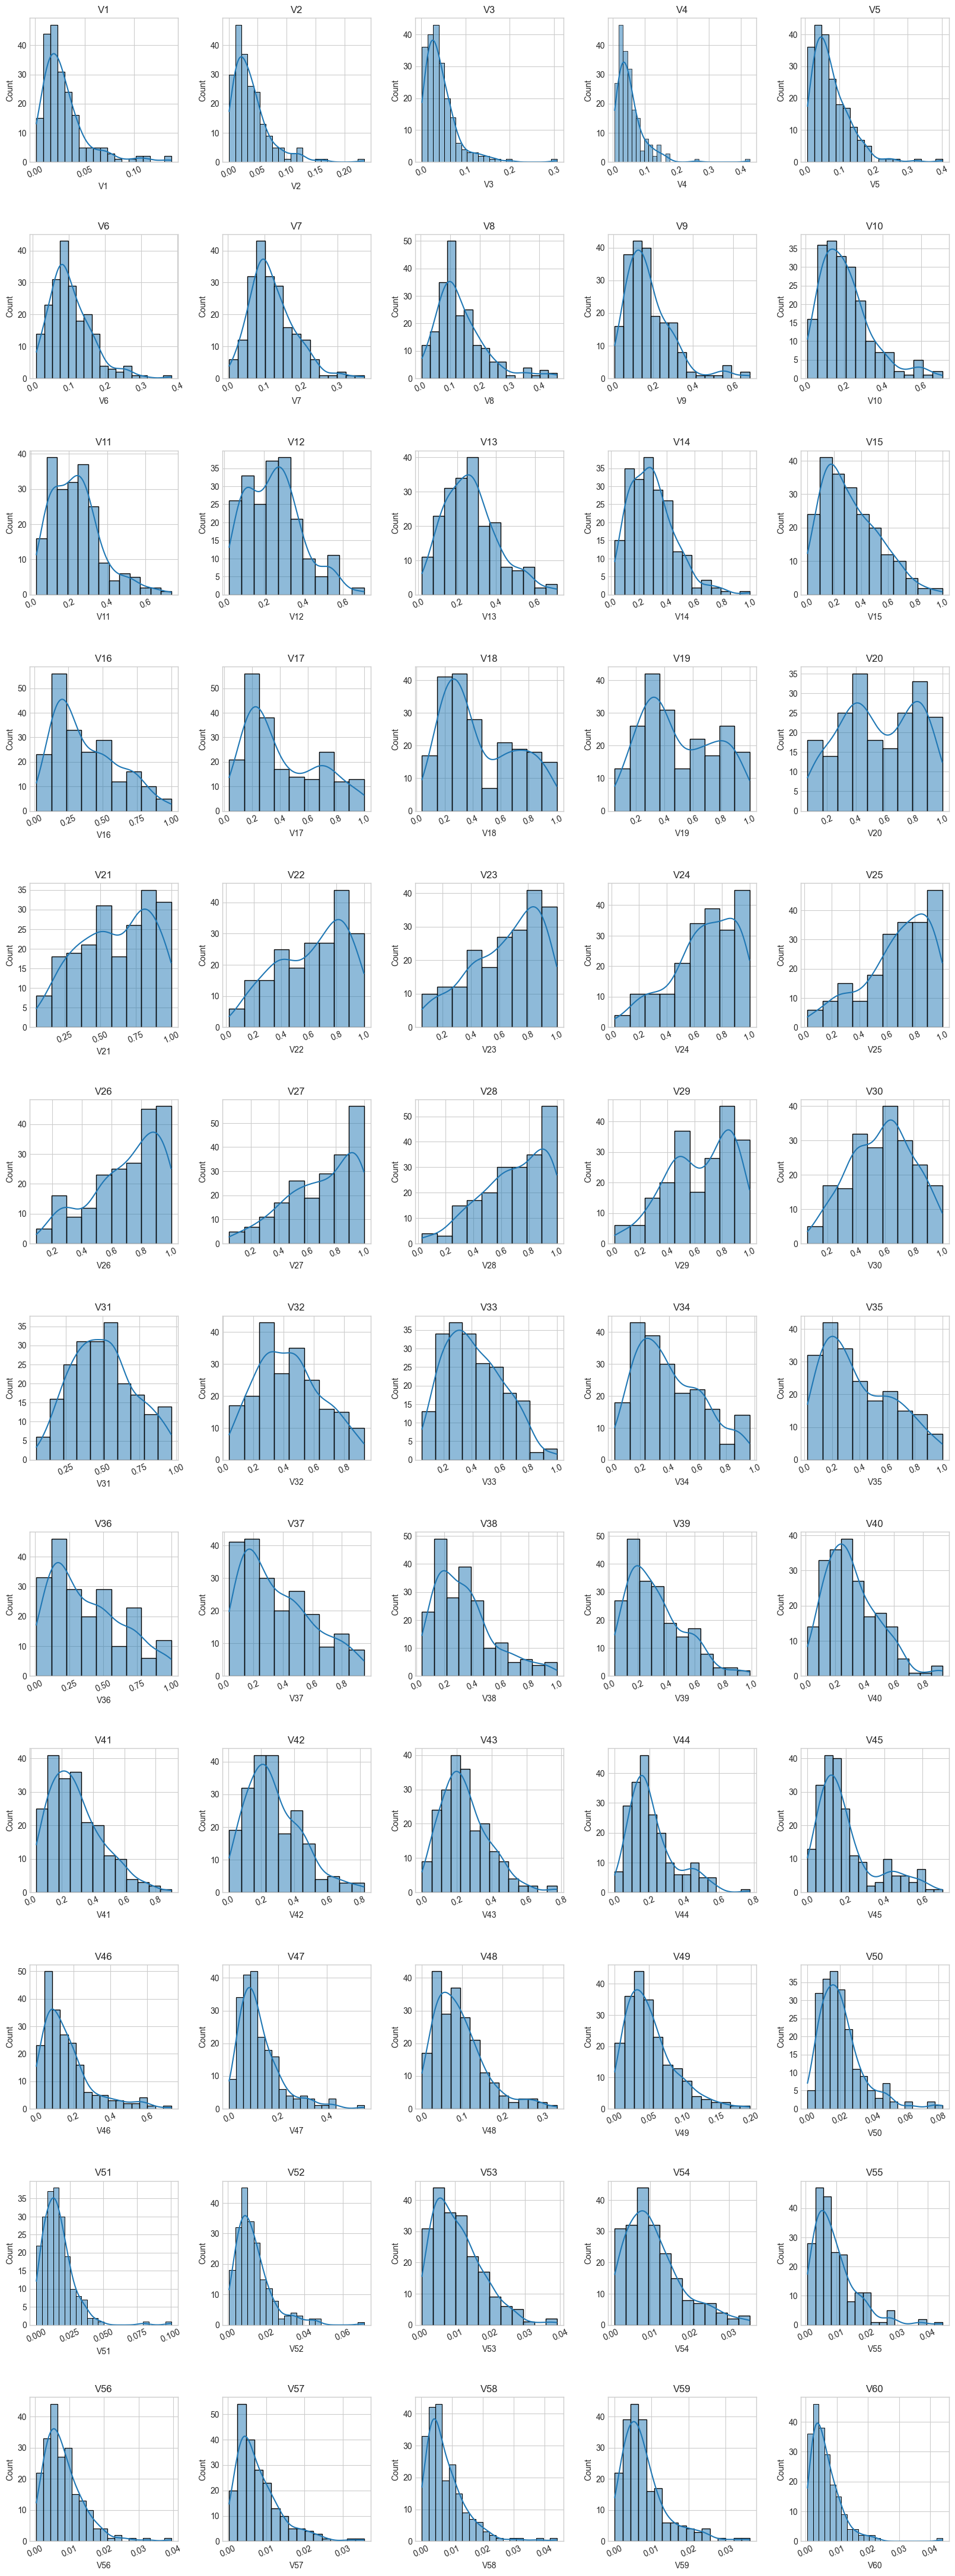
\includegraphics[scale=0.2]{histogram.png}
        \caption{Histogram của từng biến}
        \label{fig:histogram}
    \end{figure}

    Hình \ref{fig:histogram} biểu diễn histogram của từng biến.
    
    \begin{figure}[h!]
        \centering
        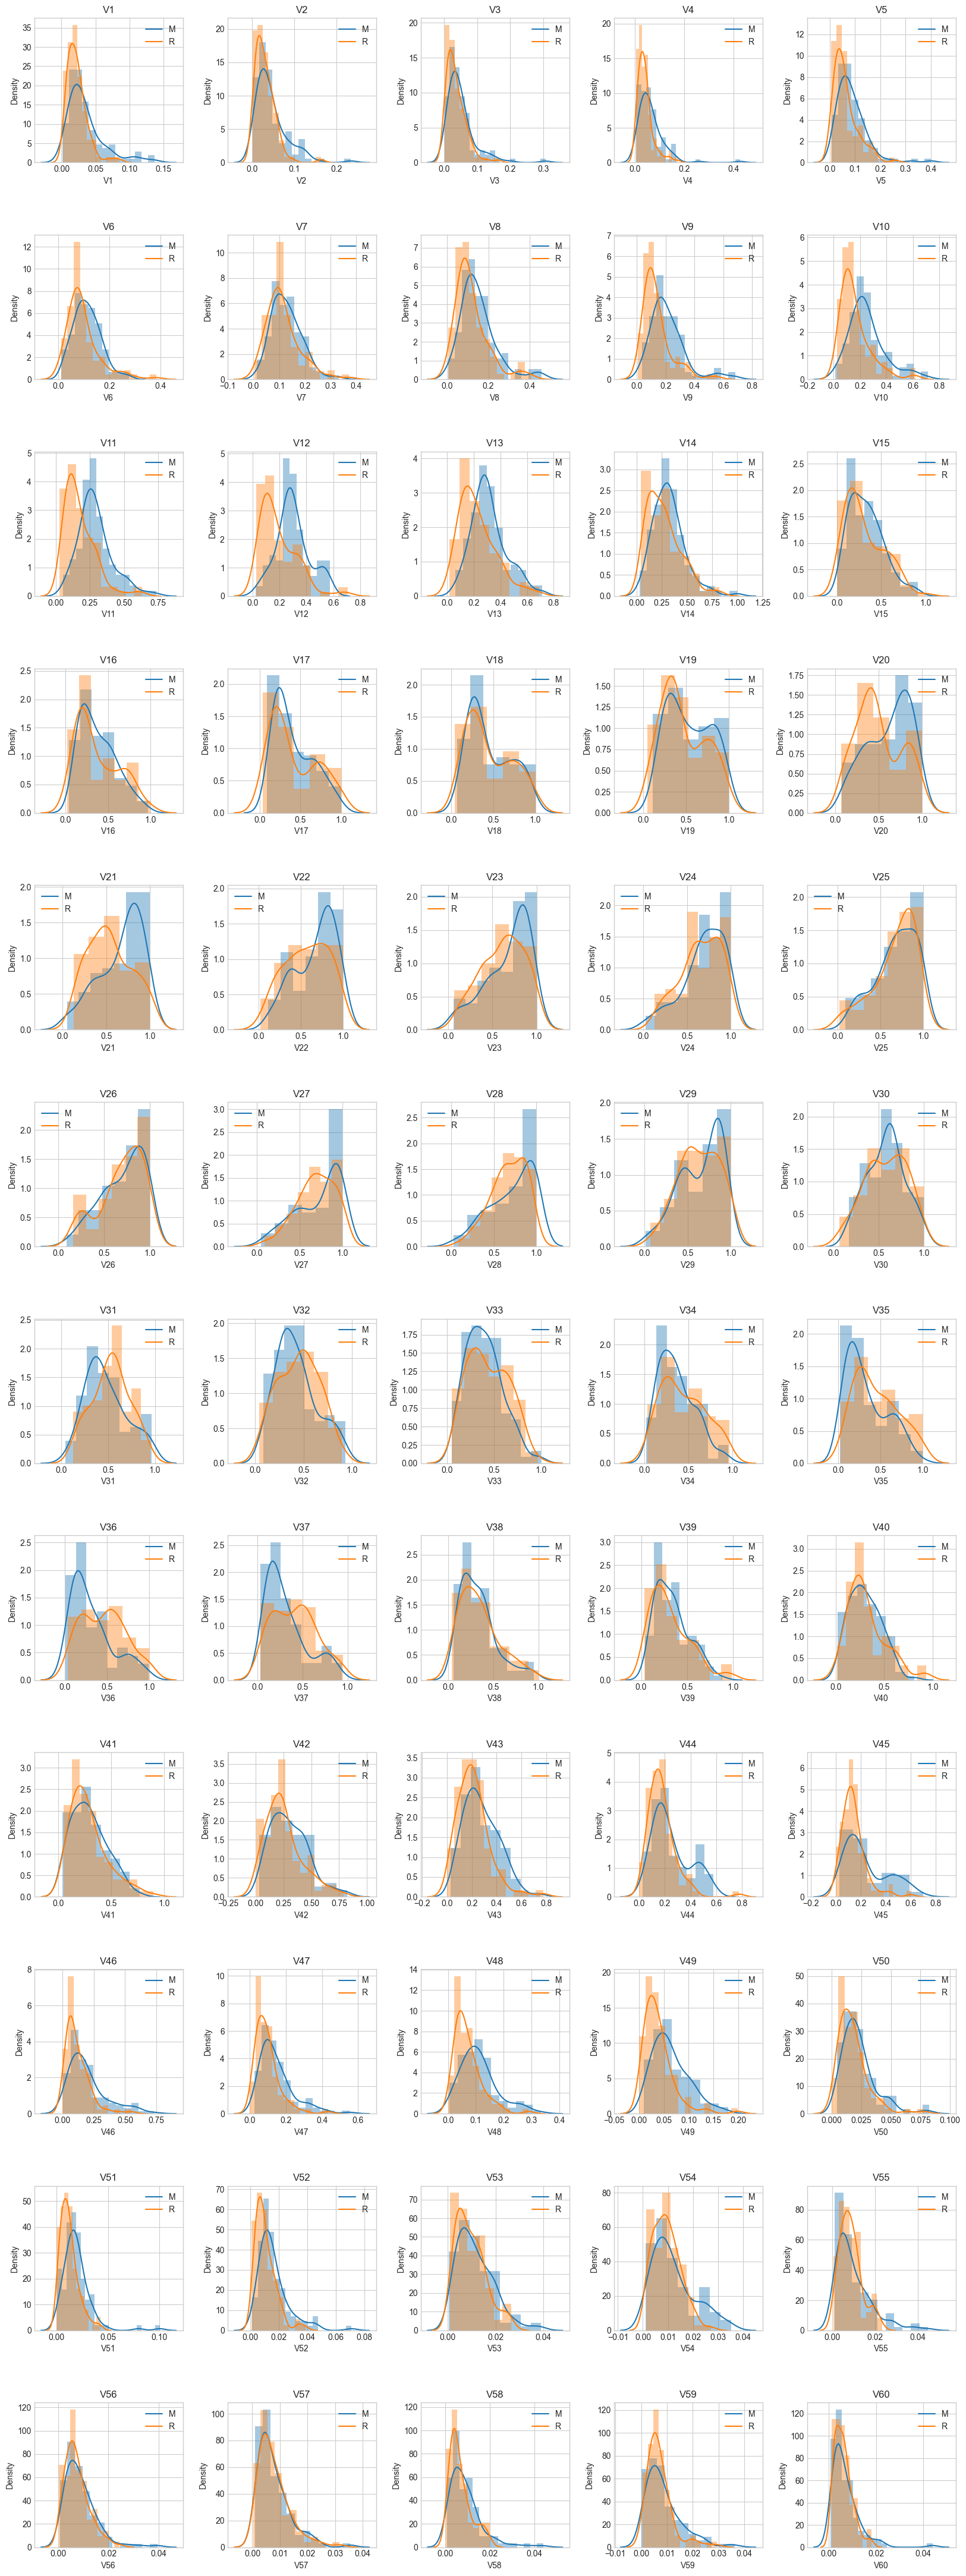
\includegraphics[scale=0.2]{figures/histogram_against_label.png}
        \caption{Histogram của từng biến có phân biệt nhãn}
        \label{fig:histogram_against_label}
    \end{figure}

    Hình \ref{fig:histogram_against_label} biểu diễn histogram của từng biến theo từng loại vật liệu của hình trụ.
    Đa phần histogram của từng biến theo từng loại vật liệu không khác nhau quá nhiều trừ các biến: V11, V12, V13, V20, V21, V48, V49, V51, V52.

\end{loigiai}

\begin{baitap}
    Hồi quy logistic có thể áp dụng cho dữ liệu Sonar để làm nhiệm vụ gì? Tại sao?
\end{baitap}

\begin{loigiai}
    Hồi quy logistic có thể áp dụng cho dữ liệu Sonar để làm nhiệm vụ gì? Tại sao?
        
    Do biến phụ thuộc của tập dữ liệu trên chỉ có hai khả năng là "M" hoặc "R".
    Nhưng ở phần mô tả thống kê, các đặc trưng không thể phân tách tuyến tính với theo từng lớp, vì vậy ta cần một bộ dự đoán kết hợp các đặc trưng (có thể chỉ cần một tập con các đặc trưng trong tập dữ liệu) và đầu ra là xác suất dự đoán rơi vào khả năng nào.
    Hay bộ dự đoán có dạng:

    \begin{equation*}
        p(y \vert \bold{x}) = f(\bold{x}) = \sigma(w_0 + w_1 x_1 + w_2 x_2 + \dots w_n x_n) = \sigma(\bold{w}^T \bold{x})
    \end{equation*}

    với:
        
    \begin{equation*}
        \begin{aligned}
            p(y \vert \bold{x}) = \sigma(\bold{w}^T \bold{x}) &= \dfrac{1}{1 + \exp(-\bold{w}^T \bold{x})} \\
            \bold{w} &= \begin{bmatrix}
                w_0 & w_1 & w_2 & \dots & w_n
            \end{bmatrix}^T \\
            \bold{x} &= \begin{bmatrix}
                1 & x_1 & x_2 & \dots & x_n
            \end{bmatrix}^T
        \end{aligned}
    \end{equation*}

    và $n (n \leq 60)$ là số đặc trưng được chọn đưa vào mô hình, $\bold{x}$ có thể là một tập con các đặc trưng từ bộ dữ liệu gốc hoặc là các đặc trưng là kết quả của kỹ trích xuất đặc trưng.

    Mô hình trên chính là mô hình hồi quy Logistic. 
    Mô hình hồi quy Logistic có thể dùng để dự đoán loại vật liệu của hình trụ phát ra tín hiệu Sonar là "M" hay "R" dựa vào đặc trưng được trích chọn hoặc trích xuất từ các đặc trưng gốc là năng lượng của các dải tần số nhất định.
    Ngoài ra ta có thể sử dụng mạng neuron nhiều lớp ẩn để dự đoán loại vật liệu của hình trụ phát ra tín hiệu Sonar.
\end{loigiai}

\begin{baitap}
    Phát biểu mô hình logistic, điều kiện của mô hình, và giải thích các ước lượng tìm được.
\end{baitap}

\begin{loigiai}
    \begin{itemize}
        \item Phát biểu mô hình logistic:
        Mô hình logistic, còn được gọi là hồi quy logistic, là một mô hình thống kê được sử dụng để dự đoán và phân loại các biến phụ thuộc nhị phân, tức là các biến có giá trị chỉ là 0 hoặc 1. 
        Mô hình này sử dụng hàm logistic để ước lượng xác suất xảy ra của biến phụ thuộc dựa trên giá trị của các biến độc lập.
        Vì kết quả là một xác suất nên kết quả đầu ra của mô hình là một số nằm trong khoảng từ 0 đến 1.
        Trong hồi quy logistic, phép biến đổi logit thường được áp dụng trên tỷ lệ giữa khả năng xảy ra trên khả năng không xảy ra được biểu diễn bằng công thức sau:

        \begin{equation*}
            \log \dfrac{p}{1-p} = w_0 +  w_1 x_1 + w_2 x_2 + \dots w_n x_n = \bold{w}^T \bold{x}
        \end{equation*}

        Trong công thức trên $p$ là biến phụ thuộc hay biến kết quả và $x$ là các biến độc lập.
        Các trọng số $\bold{w}$ là các tham số được ước lượng bằng ước hợp hợp lý cực đại MLE (Maximum Likelihood Estimation).
        Phương pháp này sử dụng một vòng lặp để cực đại hóa hàm MLE bằng cách điều chỉnh các trọng số $\bold{x}$.
        Sau khi ta tìm được các trọng số tối ưu $\bold{w}^*$, xác suất có điều kiện cho từng quan sát có thể được tính toán.
        Ta có thể chọn ngưỡng, ví dụ với ngưỡng 0.5, nếu đầu ra của mô hình nhỏ hơn 0.5, ta sẽ dự đoán 0 trong khi đầu ra lớn hơn hoặc bằng 0.5, ta sẽ dự đoán là 1.

        \item Các điều kiện của mô hình logistic:
        
        \begin{itemize}
            \item Mô hình logistic yêu cầu biến phụ thuộc có dạng nhị phân hoặc biến phụ thuộc là dạng định danh.
            \item Mô hình logistic yêu cầu các quan sát phải độc lập với nhau. Nghĩa là mỗi ví dụ học không phụ thuộc vào bất kỳ ví dụ học nào khác trong tập dữ liệu.
            Nhưng giả định này thường hay bị vi phạm do có nhiều điểm dữ liệu được đo trong một khoảng thời gian, không gian gần nhau dẫn đến các quan sát có sự liên quan nhất định với nhau.
            \item Mô hình logistic đòi hỏi phải có ít hoặc không có đa cộng tuyến giữa các biến độc lập.
            Điều này có nghĩa là các biến độc lập không nên có tương quan quá cao với nhau.
            \item Không có các điểm ngoại lai: hồi quy logistic rất nhạy cảm với các giá trị ngoại lai hoặc các điểm dữ liệu có giá trị lớn hoặc nhỏ bất thường.
            \item Mô hình logistic giả định mối quan hệ của hàm log cơ số tự nhiên của tỷ số xác suất xảy ra - không xảy ra phụ thuộc tuyến tính vào các biến độc lập.
            \item Mô hình logistic cần một số lượng các ví dụ học đủ lớn. Số ví dụ học cần ít nhất là khoảng 10 lần số biến độc lập được đưa vào mô hình.
        \end{itemize}

        \item Giải thích các ướng lượng tìm được:
        Đối với mô hình hồi quy logistic có dạng:
        \begin{equation*}
            p(y \vert \bold{x}) = f(\bold{x}) = \sigma(w_0 + w_1 x_1 + w_2 x_2 + \dots w_n x_n) = \sigma(\bold{w}^T \bold{x})
        \end{equation*}

        việc tính $\exp(w_i)$ sử dụng để chuyển đổi thành tỷ lệ giữa khả năng xảy ra 1 - không xảy ra 1.
        Nếu tỷ lệ này lớn hơn 1, thì sự kiện 1 có khả năng xảy ra cao hơn.
        Nếu tỷ lệ này nhỏ hơn 1, thì sự kiện 0 có khả năng xảy ra cao hơn.
        Dựa trên phương trình trên, tỷ lệ thay đổi theo $\exp(w_i)$ lần khi $x_i$ tăng lên 1 đơn vị.

        \item Xây dựng các mô hình:
        
        Để xây dựng mô hình, ta sẽ sử dụng các hướng sau:

        \begin{itemize}
            \item Mô hình bao gồm tất cả các biến (đặc trưng) từ tập dữ liệu.
            \item Mô hình bao gồm các đặc trưng được trích xuất từ thuật toán PCA giữa lại 95 \% thông tin.
            \item Mô hình gồm các biến được chọn từ hàm step() để lựa chọn mô hình trong ngôn ngữ R.
        \end{itemize}

        Mỗi mô hình trên được tối ưu hóa siêu tham số theo hai cách:

        \begin{itemize}
            \item Chỉ tối ưu trên random\_state của mô hình logistic (cách khởi tạo mô hình).
            \item Tối ưu trên các siêu tham số random\_state, C, solver, regularization (l1, l2, elasticnet).
        \end{itemize}

        Đầu tiên ta sẽ chọn mô hình từ hàm step() trong ngôn ngữ R:

        \begin{verbatim}
min.model <- glm(Class ~ 1, family=binomial(link="logit"), train)
max.model <- glm(reformulate(paste("V", 1:60, sep=""), "Class"), family=binomial(link="logit"), train)
m.bo <- step( max.model, scope=list(lower=min.model, upper=max.model), direction="both", trace=0)
summary(m.bo)
        \end{verbatim}

        Cho kết quả mô hình forward-backward:

        \begin{verbatim}
            Coefficients:
            Estimate Std. Error z value Pr(>|z|)    
(Intercept)    9.117      2.730   3.340 0.000839 ***
V2           -30.162     17.764  -1.698 0.089521 .  
V4           -23.301     11.428  -2.039 0.041460 *  
V10           12.587      6.618   1.902 0.057184 .  
V11          -21.339      7.066  -3.020 0.002527 ** 
V17            4.127      2.048   2.015 0.043877 *  
V20           -8.006      4.754  -1.684 0.092157 .  
V21            9.519      6.162   1.545 0.122408    
V22           -8.020      3.220  -2.491 0.012736 *  
V29            1.662      2.733   0.608 0.543130    
V30          -13.146      5.247  -2.505 0.012235 *  
V31           13.825      5.609   2.465 0.013700 *  
V32           -9.114      3.887  -2.345 0.019038 *  
V34            8.421      3.814   2.208 0.027256 *  
V35          -10.990      5.391  -2.038 0.041502 *  
V36            8.886      3.634   2.445 0.014480 *  
V49          -54.066     18.196  -2.971 0.002965 ** 
...
Residual deviance:  77.999  on 108  degrees of freedom
AIC: 114
        \end{verbatim}

        Ta thực hiện chọn mô hình theo cách forward:

        \begin{verbatim}
m.f <- step( min.model, scope=list(lower=min.model, upper=max.model), direction="forward", trace=0)
summary(m.f)
        \end{verbatim}
        
        \begin{verbatim}
            Coefficients:
            Estimate Std. Error z value Pr(>|z|)    
(Intercept)   18.301      6.755   2.709 0.006739 ** 
V11            2.153      9.678   0.222 0.823926    
V47          -29.234     14.697  -1.989 0.046687 *  
V36           19.518     10.433   1.871 0.061371 .  
V45          -19.450      8.288  -2.347 0.018931 *  
V4           -28.292     14.848  -1.905 0.056719 .  
V15          -12.549      8.760  -1.433 0.151989    
V21           -3.502      3.680  -0.952 0.341321    
V51         -201.297     88.769  -2.268 0.023350 *  
V8            15.887     11.295   1.407 0.159552    
V49         -194.056     56.475  -3.436 0.000590 ***
V50          457.951    137.282   3.336 0.000850 ***
V1          -127.995     45.281  -2.827 0.004703 ** 
V3           121.510     35.801   3.394 0.000689 ***
V52          -40.725     79.040  -0.515 0.606383    
...
Residual deviance:  62.929  on 172  degrees of freedom
AIC: 134.93
        \end{verbatim}

        Ta thực hiện chọn mô hình theo cách backward:

        \begin{verbatim}
m.b <- step( max.model, scope=list(lower=min.model, upper=max.model), direction="backward", trace=0)
summary(m.b)
        \end{verbatim}

        \begin{verbatim}
            Coefficients:
            Estimate Std. Error z value Pr(>|z|)
(Intercept)     6927     533121   0.013    0.990
V1            -21529    2447105  -0.009    0.993
V3              9013    1308937   0.007    0.995
V7              3715     292937   0.013    0.990
V9             -1717     109290  -0.016    0.987
V12            -6742     229137  -0.029    0.977
V13             3275     152052   0.022    0.983
V14            -1989     126171  -0.016    0.987
V16             3303     364286   0.009    0.993
V17             2742     116496   0.024    0.981
V18            -5149     427968  -0.012    0.990
V19             2930     331397   0.009    0.993
V20            -7113     598394  -0.012    0.991
V21             7124     473281   0.015    0.988
V22            -9118     502718  -0.018    0.986
...
Residual deviance: 2.8481e-06  on 170  degrees of freedom
AIC: 76
        \end{verbatim}

        Ta nhận thấy Wald test kiểm định các hệ số tương ứng với các biến không đóng góp trong mô hình.
        Thế nhưng đây là hiệu ứng Hauck-Donner khiến cho Wald test bị thất bại, tính toán kết quả làm cho một biến không đóng góp vào mô hình.
        Để kiểm định các hệ số trong trường hợp này, ta cần sử dụng likelihood ratio test:

        \begin{verbatim}
anova(m.b, test="Chisq")
        \end{verbatim}

        Cho kết quả:

        \begin{verbatim}
Df	Deviance	Resid. Df	Resid. Dev	Pr(>Chi)
NULL	NA	NA	207	2.874062e+02	NA
V1	1	17.713882964	206	2.696923e+02	2.567460e-05
V3	1	0.605538874	205	2.690868e+02	4.364725e-01
V7	1	0.401073639	204	2.686857e+02	5.265353e-01
V9	1	16.415841846	203	2.522699e+02	5.085840e-05
V12	1	18.464018055	202	2.338059e+02	1.731425e-05
V13	1	0.040230414	201	2.337656e+02	8.410307e-01
V14	1	1.482925834	200	2.322827e+02	2.233173e-01
V16	1	2.775377941	199	2.295073e+02	9.572406e-02
V17	1	0.040139972	198	2.294672e+02	8.412072e-01
V18	1	2.554980373	197	2.269122e+02	1.099472e-01
V19	1	9.888496760	196	2.170237e+02	1.663152e-03
V20	1	0.100063203	195	2.169236e+02	7.517538e-01
V21	1	8.718785951	194	2.082049e+02	3.149477e-03
V22	1	4.578958193	193	2.036259e+02	3.236689e-02
V23	1	0.688625865	192	2.029373e+02	4.066322e-01
V24	1	0.007890769	191	2.029294e+02	9.292170e-01
V25	1	0.173935050	190	2.027554e+02	6.766380e-01
V27	1	1.067674920	189	2.016878e+02	3.014712e-01
V29	1	1.307537307	188	2.003802e+02	2.528410e-01
V30	1	0.037764676	187	2.003425e+02	8.459164e-01
V31	1	7.187290937	186	1.931552e+02	7.342175e-03
V32	1	4.891994149	185	1.882632e+02	2.698150e-02
V33	1	6.664572192	184	1.815986e+02	9.834826e-03
V34	1	2.380619623	183	1.792180e+02	1.228488e-01
V37	1	5.647405508	182	1.735706e+02	1.748122e-02
V39	1	3.342750615	181	1.702278e+02	6.750168e-02
V40	1	0.003614541	180	1.702242e+02	9.520592e-01
V41	1	8.616473888	179	1.616077e+02	3.331361e-03
V42	1	4.215551288	178	1.573922e+02	4.005505e-02
V43	1	2.942413740	177	1.544498e+02	8.628171e-02
V46	1	12.732911806	176	1.417169e+02	3.592767e-04
V48	1	18.532618731	175	1.231842e+02	1.670213e-05
V50	1	11.198645365	174	1.119856e+02	8.185707e-04
V51	1	13.815457905	173	9.817014e+01	2.016702e-04
V52	1	24.175881404	172	7.399426e+01	8.792654e-07
V57	1	0.196456219	171	7.379781e+01	6.575966e-01
V58	1	73.797803271	170	2.848136e-06	8.654286e-18
        \end{verbatim}
    \end{itemize}

    Ta nhận thấy nếu sử dụng likelihood ratio test thì đa số các biến đóng góp đáng kể trong mô hình.

    Ta kiểm tra đồ thị Q-Q Plot của quantile residual:

    \begin{figure}[h!]
        \centering
        \begin{subfigure}[b]{\textwidth}
            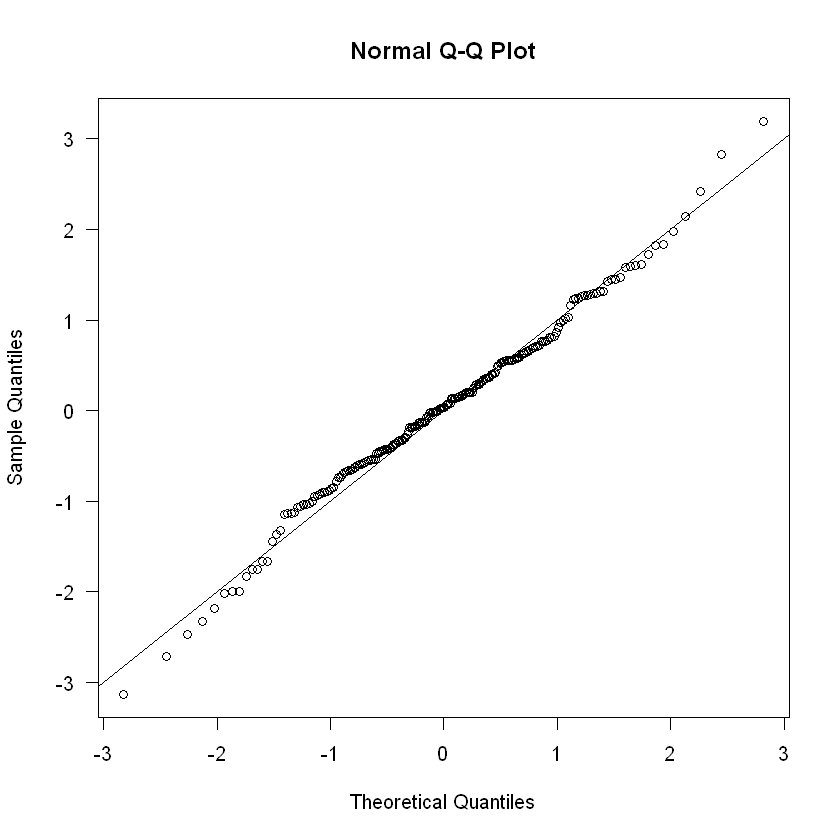
\includegraphics[width=0.3\textwidth]{figures/mf_quantile_resid.png}
            \caption{Quantile residual của mô hình forward}
        \end{subfigure}
        \hfill
        \begin{subfigure}[b]{\linewidth}
            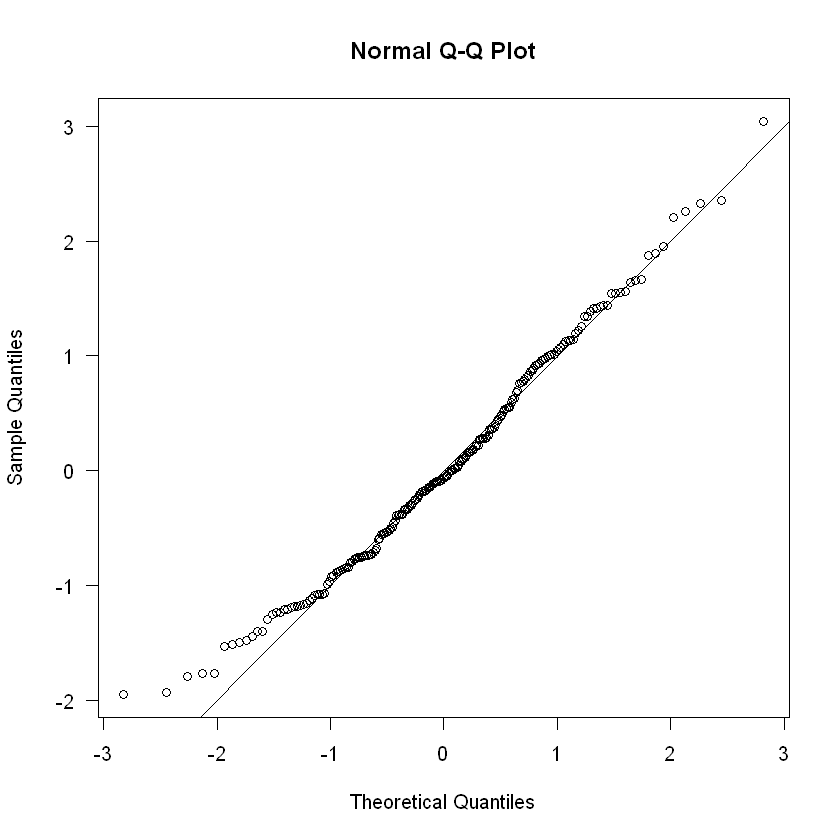
\includegraphics[width=0.3\linewidth]{figures/mb_quantile_resid.png}
            \caption{Quantile residual của mô hình backward}
        \end{subfigure}
        \hfill
        \begin{subfigure}[b]{\textwidth}
            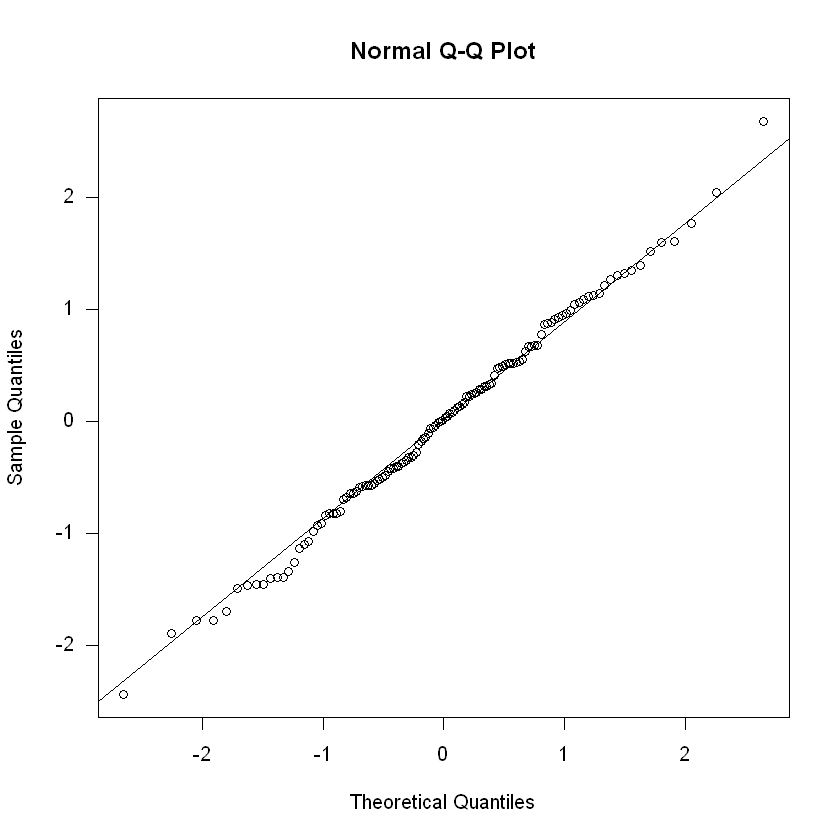
\includegraphics[width=0.3\linewidth]{figures/mbo_quantile_resid.png}
            \caption{Quantile residual của mô hình forward-backward}
        \end{subfigure}
        \caption{Quantile residual của các mô hình}
        \label{fig:Quantile-residual}
    \end{figure}
    Từ hình \ref{fig:Quantile-residual} ta nhận thấy các quantile residual của các mô hình đều có phân phối chuẩn nhưng hai bên đuôi hơi dài.Ta
    Ta kiểm tra thành phần quantile residual với giá trị $\eta$ là log của hàm tỷ số giữa sự kiện xảy ra - không xảy ra:

    \begin{figure}[h!]
        \centering
        \begin{subfigure}[b]{\textwidth}
            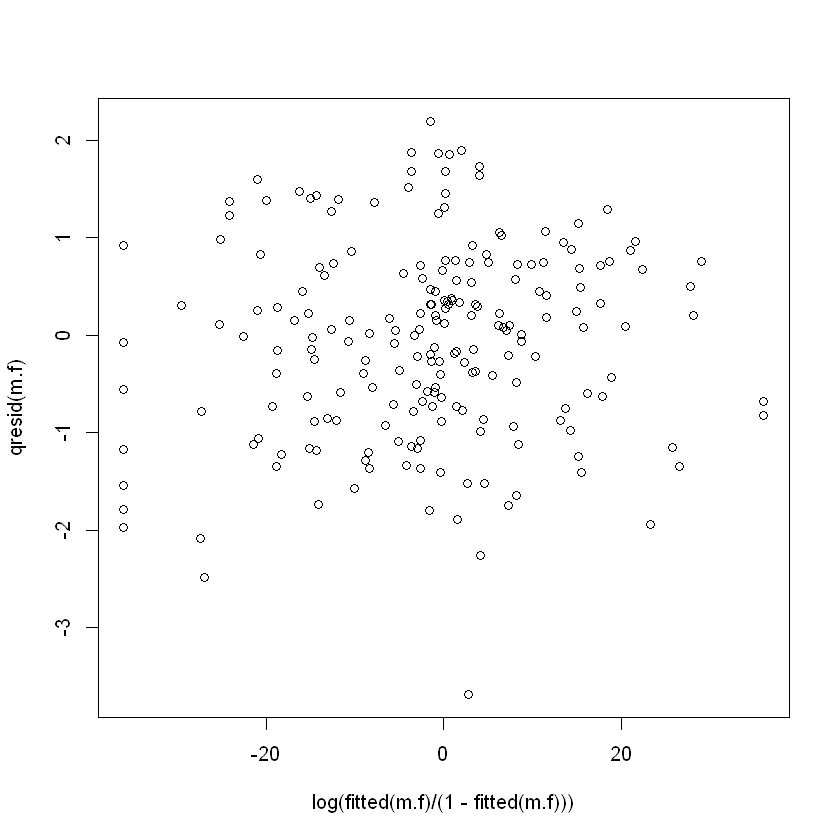
\includegraphics[width=0.3\textwidth]{figures/mf_fitted.png}
            \caption{Quantile residual của mô hình forward}
        \end{subfigure}
        \hfill
        \begin{subfigure}[b]{\linewidth}
            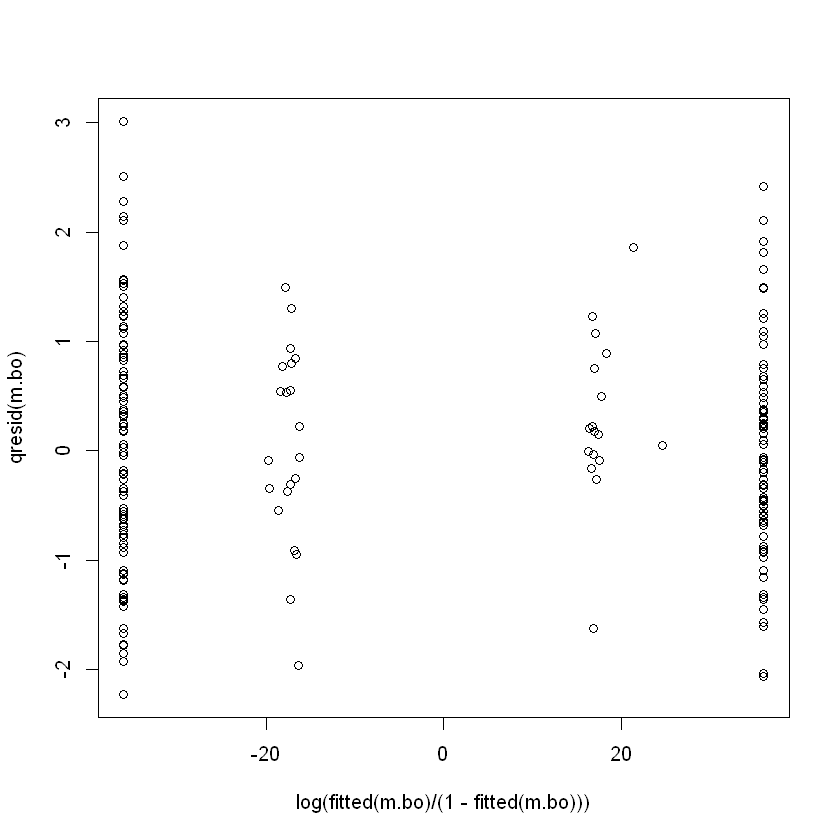
\includegraphics[width=0.3\linewidth]{figures/mb_fitted.png}
            \caption{Quantile residual của mô hình backward}
        \end{subfigure}
        \hfill
        \begin{subfigure}[b]{\textwidth}
            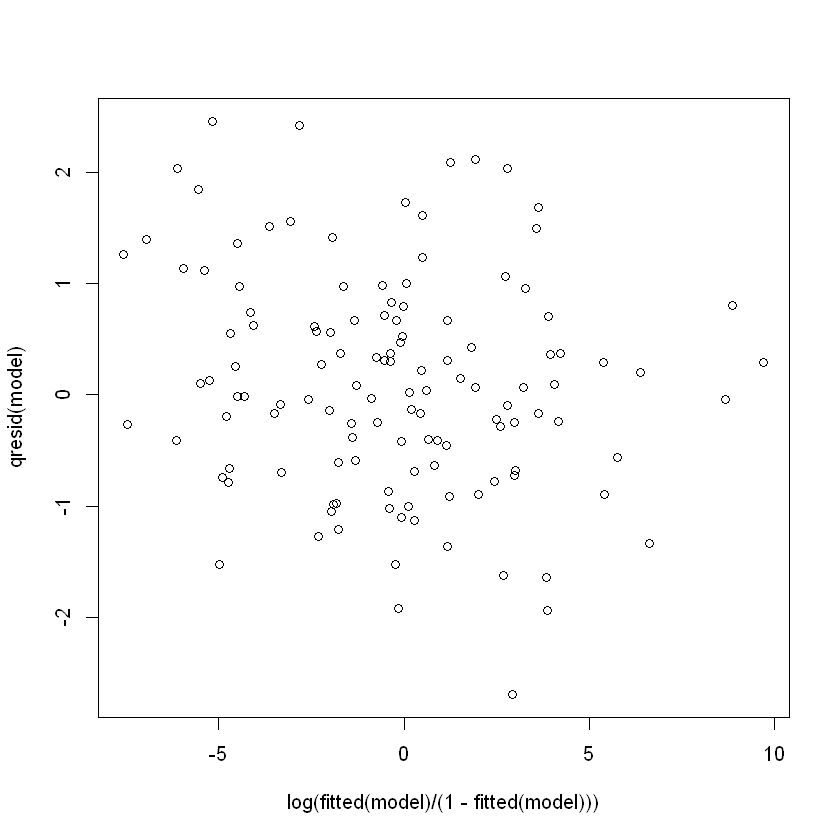
\includegraphics[width=0.3\linewidth]{figures/mbo_fitted.png}
            \caption{Quantile residual của mô hình forward-backward}
        \end{subfigure}
        \caption{Quantile residual vẽ theo các giá trị $\eta$ (hàm log-odd) của các mô hình}
        \label{fig:Quantile-fitted}
    \end{figure}

    Từ hình \ref{fig:Quantile-fitted} ta thấy mô hình forward và mô hình forward-backward thể hiện khá tốt các giả định lý thuyết khi mà quantile residual ngẫu nhiên xung quanh điểm 0 và so với giá trị $\eta$ (log-odd) của mô hình.
    Tuy nhiên mô hình backward các giá trị lại tập trung về hai phía của $\eta$ lý do là vì các tham số tương ứng với từng biến của mô hình backward quá lớn khiến cho giá trị $\eta$ phân lớp rõ ràng trở nên rất lớn hoặc rất nhỏ.

    \begin{figure}[h!]
        \centering
        \begin{subfigure}[b]{\textwidth}
            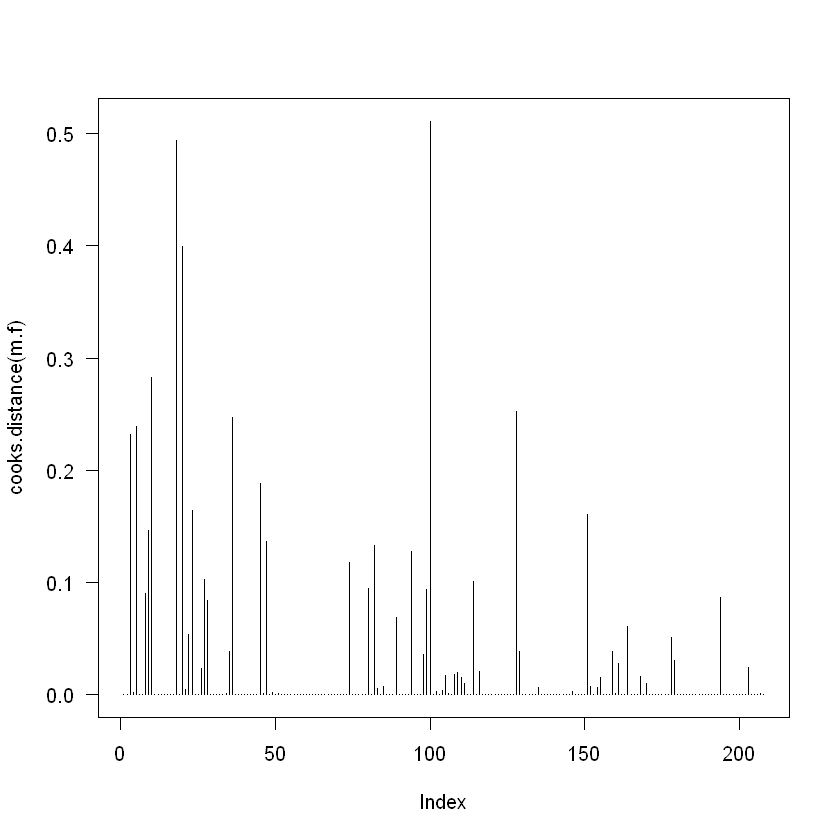
\includegraphics[width=0.3\textwidth]{figures/mf_cooks.png}
            \caption{Cooks distance của mô hình forward}
        \end{subfigure}
        \hfill
        \begin{subfigure}[b]{\linewidth}
            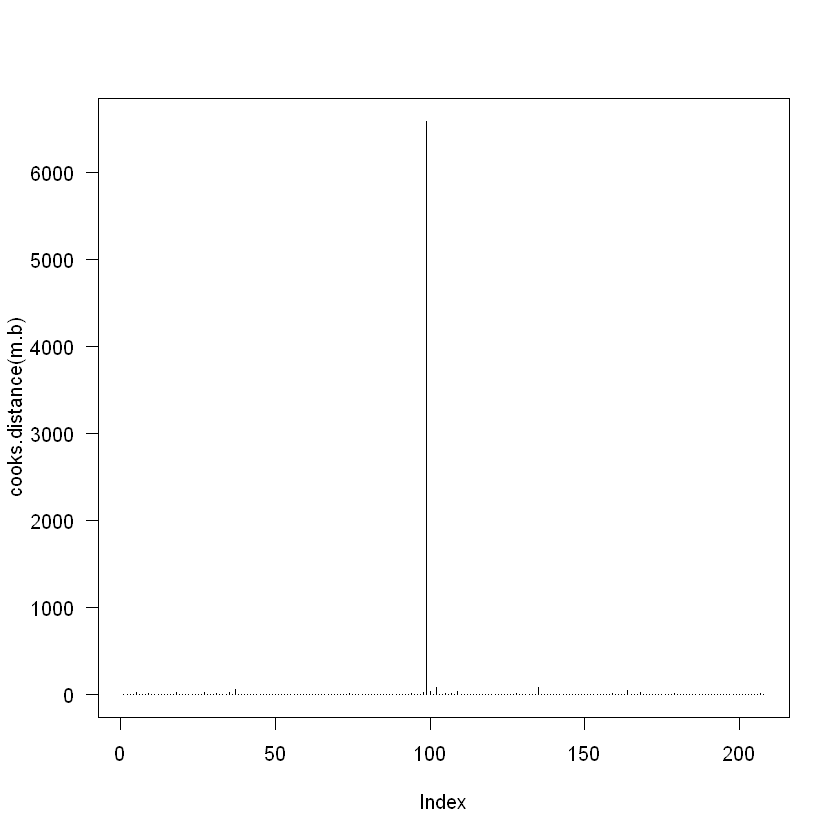
\includegraphics[width=0.3\linewidth]{figures/mb_cooks.png}
            \caption{Cooks distance của mô hình backward}
        \end{subfigure}
        \hfill
        \begin{subfigure}[b]{\textwidth}
            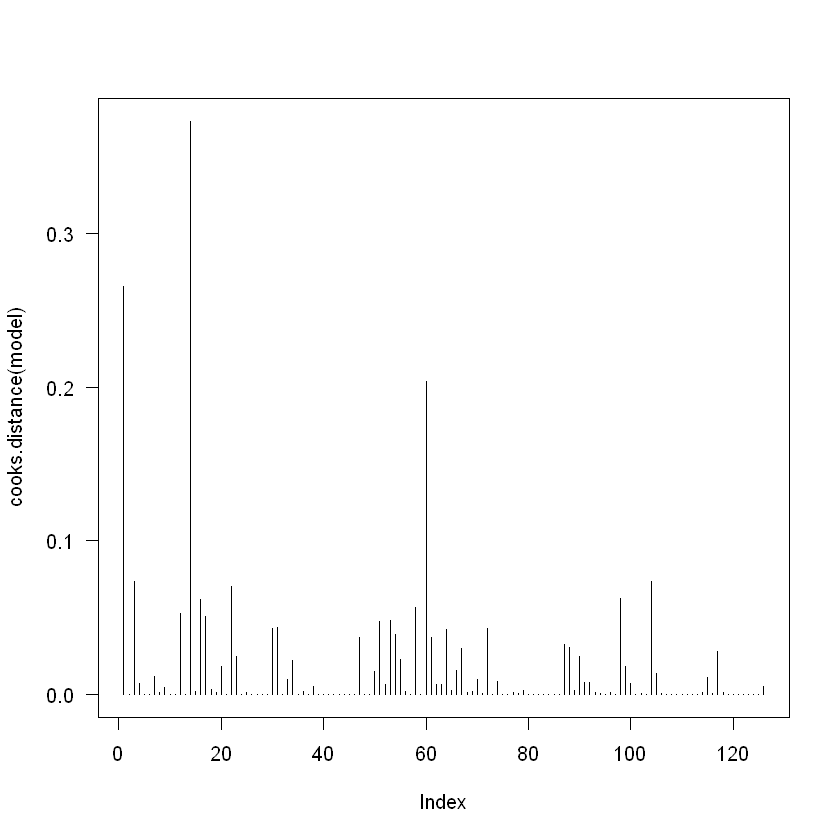
\includegraphics[width=0.3\linewidth]{figures/mbo_cooks.png}
            \caption{Cooks distance của mô hình forward-backward}
        \end{subfigure}
        \caption{Quantile residual vẽ theo các giá trị $\eta$ (hàm log-odd) của các mô hình}
        \label{fig:Cooks}
    \end{figure}
    
    Ta kiểm tra các điểm ngoại lai tương ứng với các mô hình bằng hình \ref{fig:Cooks}, theo lý thuyết thống kê một điểm được gọi là ngoại lai nếu Cooks distance lớn hơn phân vị mức 0.5 của phân phối Fisher(p, n-p).
    Ta tính phân vị mức của các mô hình trên rơi vào khoảng 0.98.
    Như vậy mô hình forward và mô hình forward-backward không có điểm ngoại lai nào nhưng mô hình backward lại có điểm ngoại lai.

    Sau khi lựa chọn các mô hình xong, ta sẽ thực hiện huấn luyện và so sánh các mô hình trên thư viện sklearn.
    Ta huấn luyện 5 mô hình:

    \begin{itemize}
        \item Mô hình gồm tất cả các biến
        \item Mô hình forward được chọn ở trên
        \item Mô hình backward được chọn ở trên
        \item Mô hình forward-backward được chọn ở trên
        \item Mô hình các biến được trích xuất từ thuật toán PCA giữ lại 95 \% thông tin
    \end{itemize}

    Mỗi mô hình trên được tối ưu hóa siêu tham số theo hai cách:

    \begin{itemize}
        \item Tìm random\_state tối ưu của mô hình logistic (cách khởi tạo mô hình).
        \item Tối ưu trên các siêu tham số random\_state, C, solver, regularization (l1, l2, elasticnet).
    \end{itemize}

    Tập dữ liệu được chia thành hai phần train và test với tỷ lệ 60 \% - 40 \%.
    Các mô hình được tối ưu hóa tham số theo cách 1 - tìm random\_state tối ưu của mô hình logistic.
    Các ký pháp của các mô hình là:

    \begin{itemize}
        \item full\_val: Mô hình gồm tất cả các biến, tìm siêu tham số sao cho chỉ số auc trên tập test là lớn nhất
        \item full\_cross\_val: Mô hình gồm tất cả các biến, tìm siêu tham số sao cho chỉ số auc trung bình trong K-Fold là lớn nhất.
        \item pca\_95\_val: Mô hình các biến được trích xuất từ thuật toán PCA giữ lại 95 \% thông tin, tìm siêu tham số sao cho chỉ số auc trên tập test là lớn nhất.
        \item pca\_95\_cross\_val: Mô hình các biến được trích xuất từ thuật toán PCA giữ lại 95 \% thông tin, tìm siêu tham số sao cho chỉ số auc trung bình trong K-Fold là lớn nhất.
        \item bo: Mô hình forward-backward được chọn ở trên, tìm siêu tham số sao cho chỉ số auc trên tập test là lớn nhất
        \item f: Mô hình forward được chọn ở trên, tìm siêu tham số sao cho chỉ số auc trên tập test là lớn nhất
        \item b: Mô hình backward được chọn ở trên, tìm siêu tham số sao cho chỉ số auc trên tập test là lớn nhất
    \end{itemize}

    Lý do phương pháp tìm siêu tham số K-Fold Cross Validation ít sử dụng trong bài tập này vì quá trình tìm siêu tham số với phương pháp K-Fold Cross Validation khá tốn kém thời gian và dù kết quả cao trên các fold nhưng khi thực hiện trên tập test kết quả vẫn khá thấp.

    Ta sử dụng một số hàm tiện ích như thực hiện thuật toán PCA:

    \begin{python}
def pca(x: np.ndarray, alpha: float=0.95) -> Tuple[np.ndarray, np.ndarray]:
    
    mu = np.mean(x, axis=0, keepdims=True)

    x_mu = x - mu

    cov_matrix = np.matmul(x_mu.T, x_mu) / x.shape[0]

    w, v = np.linalg.eig(cov_matrix)

    order = np.argsort(w)[::-1]

    w = w[order]
    v = v[:, order]

    rate = np.cumsum(w) / np.sum(w)

    r = np.where(rate >= alpha)

    U = v[:, :(r[0][0] + 1)]

    reduced_x = np.matmul(x, U)

    #print(reduced_x)

    return U, reduced_x
    \end{python}

    Hàm tính chỉ số AIC, BIC, các chỉ số này sẽ được làm chỉ số đối sánh khi chọn mô hình:

    \begin{python}
def compute_aic(y_true: np.ndarray, y_pred_prob: np.ndarray, p: int, sample_size: int=0):
    log_likelihood_elements = y_true*np.log(y_pred_prob + 1e-8) + (1-y_true)*np.log(1-y_pred_prob + 1e-8)
    if sample_size > 0:
        return -2 * sum(log_likelihood_elements) + np.log(sample_size) * p
    else:
        return -2 * sum(log_likelihood_elements) + 2 * p
    \end{python}

    
\end{loigiai}

\begin{baitap}
    Hãy dùng chỉ tiêu ROC để đánh giá về mô hình logistic tìm được ở câu 3. Đại lượng ROC đo thông tin gì của mô hình? Giải thích
\end{baitap}

\begin{loigiai}
    \begin{itemize}
        \item Đại lượng ROC đo thông tin gì của mô hình?
        
        ROC (Receiver operating characteristic) là một đồ thị được sử dụng khá phổ biến trong validation các model phân loại nhị phân. Đường cong này được tạo ra bằng cách biểu diễn tỷ lệ dự báo true positive rate (TPR) dựa trên tỷ lệ dự báo failse positive rate (FPR) tại các ngưỡng Threshold khác nhau. 
        Trong học máy ta gọi true positive rate là độ nhạy sensitivity tức là xác xuất dự báo đúng một sự kiện là positive. Tỷ lệ false positive rate là probability of false alarm (tỷ lệ cảnh báo sai, một sự kiện là negative nhưng coi nó là positive) và tỷ lệ này tương ứng với xác xuất mắc sai lầm loại II. Như vậy ROC curve sẽ thể hiện mối quan hệ, sự đánh đổi và ý nghĩa lựa chọn một model phù hợp của độ nhạy và tỷ lệ cảnh báo sai.

        Xác xuất mắc sai lầm loại I và loại II trong dự báo được nhắc đến khá nhiều trong các tài liệu thống kê học và đây là những loại sai lầm đặc trưng cơ bản trong các model dự báo. Giả sử chúng ta xét một model dự báo sự kiện với 2 khả năng positive (tích cực) và negative (tiêu cực). Các kết quả của model xảy ra sẽ rơi vào 4 nhóm sau:

        \begin{itemize}
            \item TP: True positive, dự báo đúng sự kiện là positive trong trường hợp thực tế là positive.
            \item FP: False positive, dự báo sai sự kiện là positive trong trường hợp thực tế là negative.
            \item TN: True negative, dự báo đúng sự kiện là negative trong trường hợp thực tế là negative.
            \item FN: False negative, dự báo sai sự kiện là negative trong trường hợp thực tế là positive.
        \end{itemize}

        Các chỉ số dùng trong ROC Curve:

        \begin{itemize}
            \item TPR(True Positive Rate/Sentivity/Recall) Biểu diễn tỷ lệ phân loại chính xác các mẫu dương tính trên tất cả các mẫu dương tính, được tính theo công thức:
            \begin{equation*}
                TPR = \dfrac{TP}{TP + FN}
            \end{equation*}
            TPR càng cao thì các mẫu dương tính càng được phân loại chính xác.
            \item Specificity: Biểu diễn tỷ lệ phân loại chính xác các mẫu âm tính trên tất cả các mâu âm tính, được tính theo công thức:
            \begin{equation*}
                Specificity = \dfrac{TN}{TN + FP}
            \end{equation*}
            \item FPR(False Positive Rate/Fall-out): Biểu diễn tỷ lệ gắn nhãn sai các mẫu âm tính thành dương tính trên tất cả các mẫu âm tính, được tính theo công thức:
            \begin{equation*}
                FPR = 1 - Specificity = \dfrac{FP}{TN + FP}
            \end{equation*}
        \end{itemize}
        Có thể thấy Specificity nghịch biến với FPR. FPR càng cao thì Specificity càng giảm và số lượng các mẫu âm tính bị gắn nhãn sai càng lớn.
        Thông thường các khía cạnh dự báo của một model mà chúng ta quan tâm sẽ tập trung vào 2 tỷ lệ: TPR/Sensitivity và FPR. 
        Vì vậy cần một đồ thị biểu diễn mối liên hệ giữa chúng. 
        ROC Curve là một đường cong đặc thù thể hiện các tỷ lệ này theo những ngưỡng xác suất.

        Dựa trênmô hình logistic, sau khi huấn luyện chúng ta sẽ thu được các điểm số của biến được dự báo. 
        Nếu thiết lập một điểm ngưỡng cho mô hình ta sẽ có một ngưỡng để đánh giá mô hình dự báo ra kết quả positive hay negative. 
        Đường cong ROC sẽ biểu diễn với mỗi điểm ngưỡng ứng với nó sẽ có tỷ lệ TPR/Sensitivity và FPR là bao nhiêu. 
        Trong đó trục tung ứng với tỷ lệ TPR/Sensitivity và trục hoành ứng với tỷ lệ FPR.

        Đường cong ROC là một dạng đường cong lồi hướng về phía góc trên cùng bên trái. 
        Ứng với mỗi giá trị xác suất ngưỡng cao hơn thì TPR/Sensitivity cao hơn và FPR cao hơn. Điều này có thể lý giải như sau:

        Khi các điểm xác suất tăng dần thì tỷ lệ TPR/Sensitivity giảm dần do ở mức điểm cao hơn thì số lượng được dự báo là positive có thể giảm trong khi số lượng positive thực tế không đổi vậy nên TPR/Sensitivity có thể giảm. 
        Đồng thời tỷ lệ FPR cũng giảm do mức điểm cao hơn thì số lượng dự báo là positive giảm nên số lượng được dự báo sai FP (Failse Positive) có thể giảm vì vậy FPR giảm.
        Do đó đường cong ROC có xu hướng đồng biến giữa TPR/Sensitivity và FPR.
    \end{itemize}
\end{loigiai}

\newpage
\printbibliography[title={TÀI LIỆU THAM KHẢO}]



\end{document}
